\chapter{Species and forms}
\label{chap:species}
Pokémon are partitioned into species.
Each species is identified by its own Pokédex number.
As we will see, this number is the only thing guaranteed to be shared
 among all the population of a species.

\section{Forms}
\label{chap:forms}
Some species boast multiple forms and genders, all sharing one common Pokédex entry.
Form is usually merely a visual distinction, but it is sometimes reflected
 in stats or even typing.
All Pokémon of a given form share the same Attack (ATK), Defense (DEF), and
 Stamina (STA) base statistics.
These statistics are always positive integers.

Common forms include \textit{Mega}, a temporary form with greater ATK and DEF (see \autoref{sec:mega}),
  \textit{Dynamax} and \textit{Gigantamax}, temporary forms with the ability to use
  powerful attacks (see \autoref{sec:dmax} and \autoref{sec:gmax}),
  and \textit{Shiny}, a visually distinctive and rare form (see \autoref{sec:shiny}).
Regional forms are also seen: Alolan, Galarian, Hisuian, and Paldean.
Gender, if differentiated at all, is usually a small change to
 appearance or call, but it (like other forms) also affects a few evolutionary
 paths.

\section{Evolution}
\label{chap:evolution}
Some species can, under the correct conditions, evolve into others.
We call the set of Pokémon related by evolution operations a genus.
Change of form is not an evolution, since the species remains the same.
We call a Pokémon that has undergone $N$ evolutions a Stage $N+1$ Pokémon.
No Pokémon of Stage 4 or higher currently exist.
Evolution (unlike some form changes) is irreversible.
Evolution does not necessarily preserve typing, i.e.\ typing is not always
  constant within a genus (\autoref{table:heteroevolve}).
\input{out/hetero}
Almost all evolutions require that Candy of that genus (Zygarde is an exception),
  and some evolutions depend upon some condition (\autoref{table:condevolutions})
  or catalyzing item, which is consumed (\autoref{table:itemevolutions})
Evolution generally improves base stats \textbf{(FIXME: are there exceptions?)},
  and typically makes available new, more powerful attacks.
Evolution revives a Pokémon if it is fainted, and always fully restores HP\@.

\begin{table}[ht]
\footnotesize
\begin{center}
  \begin{tabular}{lll}
    Base & Requirements & Result \\
    \Midrule
  \end{tabular}
\end{center}
\caption{Evolutions dependent upon a condition}
\label{table:condevolutions}
\end{table}

\begin{table}[ht]
\footnotesize
\begin{center}
  \begin{tabular}{lll}
    Base & Requirements & Result \\
    \Midrule \\
    Gloom & 100 Oddish candy + 
\includegraphics[width=1em,height=1em]{images/sunstone.png} & Bellossom \\
    Sunkern & 50 Sunkern candy + 
\includegraphics[width=1em,height=1em]{images/sunstone.png} & Sunflora \\
    Cottonee & 50 Cottonee candy + 
\includegraphics[width=1em,height=1em]{images/sunstone.png} & Whimsicott \\
    Petilil & 50 Petilil candy + 
\includegraphics[width=1em,height=1em]{images/sunstone.png} & Lilligant \\
    Helioptile & 50 Helioptile candy + 
\includegraphics[width=1em,height=1em]{images/sunstone.png} & Heliolisk \\
    Poliwhirl & 100 Poliwag candy + 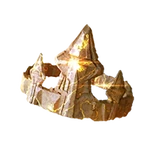
\includegraphics[width=1em,height=1em]{images/kingsrock.png} & Politoed \\
    Slowpoke & 50 Slowpoke candy + 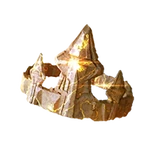
\includegraphics[width=1em,height=1em]{images/kingsrock.png} & Slowking \\
    Onix & 50 Onix candy + 
\includegraphics[width=1em,height=1em]{images/metalcoat.png} & Steelix \\
    Scyther & 50 Scyther candy + 
\includegraphics[width=1em,height=1em]{images/metalcoat.png} & Scizor \\
    Seadra & 100 Horsea candy + 
\includegraphics[width=1em,height=1em]{images/dragonscale.png} & Kingdra \\
    Porygon & 25 Porygon candy + 
\includegraphics[width=1em,height=1em]{images/upgrade.png} & Porygon2 \\
    Poygon2 & 100 Porygon candy + 
\includegraphics[width=1em,height=1em]{images/sinnohstone.png} & Porygon-Z \\
    Lickitung & 100 Lickitung Candy + 
\includegraphics[width=1em,height=1em]{images/sinnohstone.png} & Lickilicky \\
    Tangela	& 100 Tangela Candy + 
\includegraphics[width=1em,height=1em]{images/sinnohstone.png} & Tangrowth \\
    Electabuzz & 100 Elekid Candy + 
\includegraphics[width=1em,height=1em]{images/sinnohstone.png} & Electivire	\\
    Magmar & 100 Magby Candy + 
\includegraphics[width=1em,height=1em]{images/sinnohstone.png} & Magmortar	\\
    Sneasel & 100 Sneasel Candy + 
\includegraphics[width=1em,height=1em]{images/sinnohstone.png} & Weavile	\\
    Togetic & 100 Togepi Candy + 
\includegraphics[width=1em,height=1em]{images/sinnohstone.png} & Togekiss	\\
    Yanma & 100 Yanma Candy + 
\includegraphics[width=1em,height=1em]{images/sinnohstone.png} & Yanmega	\\
    Gligar & 100 Gligar Candy + 
\includegraphics[width=1em,height=1em]{images/sinnohstone.png} & Gliscor	\\
    Murkrow & 100 Murkrow Candy + 
\includegraphics[width=1em,height=1em]{images/sinnohstone.png} & Honchkrow	\\
    Male Kirlia & 100 Ralts Candy + 
\includegraphics[width=1em,height=1em]{images/sinnohstone.png} & Gallade	\\
    Misdreavus & 100 Misdreavus Candy + 
\includegraphics[width=1em,height=1em]{images/sinnohstone.png} & Mismagius	\\
    Piloswine & 100 Swinub Candy + 
\includegraphics[width=1em,height=1em]{images/sinnohstone.png} & Mamoswine	\\
    Dusclops & 100 Duskull Candy + 
\includegraphics[width=1em,height=1em]{images/sinnohstone.png} & Dusknoir	\\
    Female Snorunt & 100 Snorunt Candy + 
\includegraphics[width=1em,height=1em]{images/sinnohstone.png} & Froslass	\\
    Aipom & 100 Aipom Candy + 
\includegraphics[width=1em,height=1em]{images/sinnohstone.png} & Ambipom	\\
    Roselia & 100 Budew Candy + 
\includegraphics[width=1em,height=1em]{images/sinnohstone.png} & Roserade	\\
    Applin & 200 Applin Candy + 20 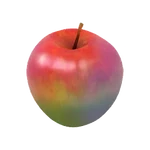
\includegraphics[width=1em,height=1em]{images/tartapple.png} & Flapple \\
    Applin & 200 Applin Candy + 20 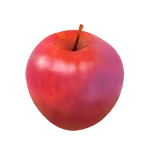
\includegraphics[width=1em,height=1em]{images/sweetapple.png} & Appletun \\
    Zygarde 10\% & 50 Zygarde Cubes & Zygarde 50\% \\
    Zygarde 50\% & 200 Zygarde Cubes & Zygarde Complete \\
  \end{tabular}
\end{center}
\caption{Evolutions dependent upon items}
\label{table:itemevolutions}
\end{table}

\subsection{Eevolution}
\begin{figure}
\end{figure}
Evolution within the Eevee genus is a complicated and unique affair.
Eevee (the species) can evolve into eight different species.
Five of these targets require some condition, and are deterministic.
If none of the conditions are met, the evolution is nondeterministic,
  with three possible results.
A second mechanism exists based on nicknames, deterministic across all eight targets,
  but it can only be used once per target per Trainer.
\textbf{FIXME: how do the two affect one another, which has priority?}
If the evolution is deterministic, the ``Evolve'' button will show the
  unique target.
It will otherwise show a question mark.
\textbf{FIXME: screenshot(s)}
Eevee's evolutions are often strong Pokémon early in the game.

For the nickname-based mechanic, give the Eevee you wish to evolve the nickname
  specified for the desired target from \autoref{table:eevee}.
\begin{table}
  \begin{center}
    \begin{tabular}{lrr}
      Target & Nickname & Condition\\
      \Midrule\\
      Vaporeon & Rainer & random\\
      Jolteon & Sparky & random\\
      Flareon & Pyro & random\\
      Sylveon & Kira & \\
      Espeon & Sakura & \\
      Umbreon & Tamao & \\
      Leafeon & Linnea & \\
      Glacion & Rea & \\
    \end{tabular}
  \end{center}
  \caption{Eevolution}
  \label{table:eevee}
\end{table}

\section{Shadow and Purified Pokémon}
Team Rocket uses ``Shadow'' Pokémon modified for more attack
 and less defense capability than their base forms (for more details,
 see \autoref{chap:damage}).
Shadow Pokémon cost 20\% more than normal to evolve, teach second charged attacks, or power up.
When captured from Team Rocket, they enter their own Shadow Pokédex.
Captured Shadow Pokémon always know the charged attack Frustration.
Only during certain special events can this charged attack be replaced,
 at which time a Charged TM is required as normal.
It's a pretty terrible Charged Attack, and this really degrades the
 Shadow Pokémon until it can be replaced.
A Shadow Pokémon can be taught a second Charged Attack at any time.
Frustration is preserved across evolution, as is Shadow status itself.
Shadow Pokémon cannot be traded.

Purification of a Shadow Pokémon has a cost in Stardust and Candy.
Purified Pokémon cost 10\% less than normal to evolve, teach second charged attacks, or power up.
Purification enters the Pokémon into its own Purified Pokédex,
 advances it to level 25 if not yet there,
 eliminates the attack bonus and defense penalty,
 replaces the primary charged attack with Return (exclusive to purified Pokémon),
 and increases each IV component by 2  (up to the usual max of 15).
Return is preserved across evolution, as is Purified status itself.
Purified Pokémon can be traded, but constitute a Special Trade (\autoref{sec:trades}).

\section{Trends among species}
\textbf{FIXME: graphs of stat distribution by type}
